% Created 2022-03-31 Thu 20:58
% Intended LaTeX compiler: pdflatex
\documentclass[11pt]{article}
\usepackage[utf8]{inputenc}
\usepackage[T1]{fontenc}
\usepackage{graphicx}
\usepackage{longtable}
\usepackage{wrapfig}
\usepackage{rotating}
\usepackage[normalem]{ulem}
\usepackage{amsmath}
\usepackage{amssymb}
\usepackage{capt-of}
\usepackage{hyperref}
\usepackage{minted}
\usepackage[margin=0.8in]{geometry}
\author{Mahan Fathi}
\date{\today}
\title{\textbf{Homework \#4}}
\hypersetup{
 pdfauthor={Mahan Fathi},
 pdftitle={\textbf{Homework \#4}},
 pdfkeywords={},
 pdfsubject={},
 pdfcreator={Emacs 27.2 (Org mode 9.6)}, 
 pdflang={English}}
\begin{document}

\maketitle
\clearpage

\section{Question 1}
\label{sec:orgf55f7cf}

\begin{figure}[htbp]
\centering
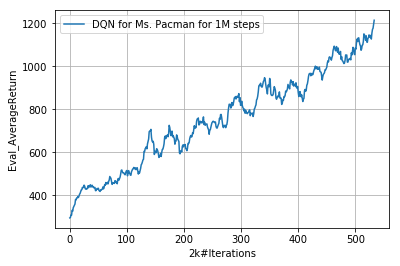
\includegraphics[width=.9\linewidth]{./1.png}
\caption{\textbf{Q1} \texttt{MsPacman-v0} Single DQN}
\end{figure}

\begin{listing}[htbp]
\begin{minted}[]{bash}
python run_hw4.py exp_name=q1 env_name=MsPacman-v0 n_iter=10000000
\end{minted}
\caption{\textbf{Q1} Run command}
\end{listing}

\clearpage

\section{Question 2}
\label{sec:org87869f4}
The plummet after reaching a total return of 150 has already been alluded to in the problem statement, and is the case also here.

\begin{figure}[htbp]
\centering
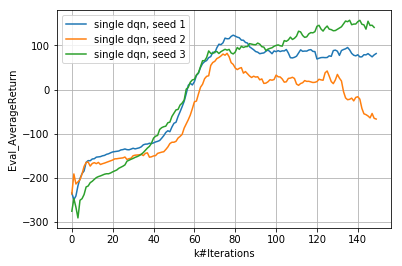
\includegraphics[width=.9\linewidth]{./21.png}
\caption{\textbf{Q2} \texttt{LunarLander-v3} Single DQN}
\end{figure}

\begin{figure}[htbp]
\centering
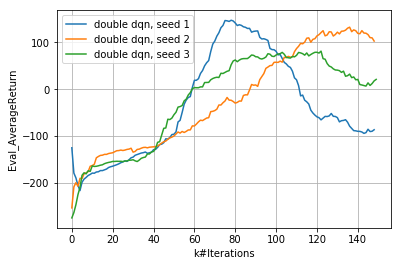
\includegraphics[width=.9\linewidth]{./22.png}
\caption{\textbf{Q2} \texttt{LunarLander-v3} Double DQN}
\end{figure}

\begin{listing}[htbp]
\begin{minted}[]{bash}
python run_hw4.py env_name=LunarLander-v3 \
    exp_name=q2_dqn_1 seed=1 n_iter=1000000 double_q=null

python run_hw4.py env_name=LunarLander-v3 \
    exp_name=q2_dqn_2 seed=2 n_iter=1000000 double_q=null

python run_hw4.py env_name=LunarLander-v3 \
    exp_name=q2_dqn_3 seed=3 n_iter=1000000 double_q=null


python run_hw4.py env_name=LunarLander-v3 \
    exp_name=q2_doubledqn_1 seed=1 n_iter=200000

python run_hw4.py env_name=LunarLander-v3 \
    exp_name=q2_doubledqn_2 seed=2 n_iter=200000

python run_hw4.py env_name=LunarLander-v3 \
    exp_name=q2_doubledqn_3 seed=3 n_iter=200000
\end{minted}
\caption{\textbf{Q2} Run commands}
\end{listing}

\clearpage

\section{Question 3}
\label{sec:org834ab6d}
\begin{figure}[htbp]
\centering
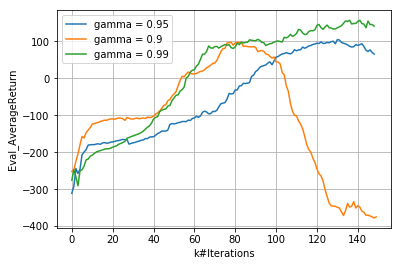
\includegraphics[width=.9\linewidth]{./3.png}
\caption{\textbf{Q3} \texttt{LunarLander-v3} with ablations for \texttt{gamma}}
\end{figure}

\begin{listing}[htbp]
\begin{minted}[]{bash}
python run_hw4.py env_name=LunarLander-v3 \
    exp_name=q3_gamma0.9 n_iter=1000000 gamma=0.9

python run_hw4.py env_name=LunarLander-v3 \
    exp_name=q3_gamma0.95 n_iter=1000000 gamma=0.95

python run_hw4.py env_name=LunarLander-v3 \
    exp_name=q3_gamma0.99 n_iter=1000000 gamma=0.99
\end{minted}
\caption{\textbf{Q3} Run commands}
\end{listing}

Here we have chosen \texttt{params['gamma']} as our ablation variable. The reason behind this is that one convenient handle we have over the bias and variance trade-off in a Q-Learning algorithm, is the discount factor. My speculation was that the fall in the return after 150 could be adressed by making the Q values more or less sensitive to the changes in the rewarding pattern of the environment. We can see from plots that indeed \(\gamma=0.99\) performs best, as it corresponds to a scenario in which the algorithm is least fixated on the current reward and takes into account the future rewards more, as opposed to other \(\gamma\) values.

\clearpage


\section{Question 4}
\label{sec:org40ff35e}

\begin{figure}[htbp]
\centering
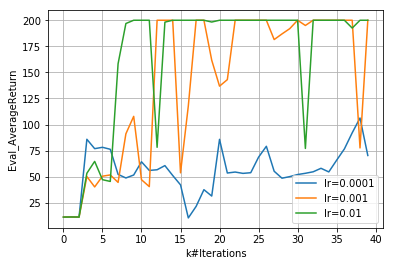
\includegraphics[width=.9\linewidth]{./41.png}
\caption{\textbf{Q4}  DDPG for \texttt{InvertedPendulum-v2}, \texttt{learning\_rate} ablations}
\end{figure}


\begin{figure}[htbp]
\centering
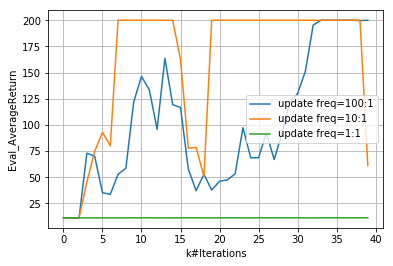
\includegraphics[width=.9\linewidth]{./42.png}
\caption{\textbf{Q4}  DDPG for \texttt{InvertedPendulum-v2}, \texttt{policy\_update\_frequency} ablations}
\end{figure}

\begin{minted}[]{bash}
python run_hw4.py exp_name=q4_ddpg_lr0.001  rl_alg=ddpg \
    env_name=InvertedPendulum-v2 atari=false n_iter=40000 learning_rate=0.001

python run_hw4.py exp_name=q4_ddpg_lr0.01   rl_alg=ddpg \
    env_name=InvertedPendulum-v2 atari=false n_iter=40000 learning_rate=0.01

python run_hw4.py exp_name=q4_ddpg_lr0.0001 rl_alg=ddpg \
    env_name=InvertedPendulum-v2 atari=false n_iter=40000 learning_rate=0.0001


python run_hw4.py exp_name=q4_ddpg_uf1   rl_alg=ddpg \
    env_name=InvertedPendulum-v2 atari=false n_iter=40000 policy_update_frequency=1

python run_hw4.py exp_name=q4_ddpg_uf10  rl_alg=ddpg \
    env_name=InvertedPendulum-v2 atari=false n_iter=40000 policy_update_frequency=10

python run_hw4.py exp_name=q4_ddpg_uf100 rl_alg=ddpg \
    env_name=InvertedPendulum-v2 atari=false n_iter=40000 policy_update_frequency=100
\end{minted}

\clearpage


\section{Question 5}
\label{sec:org7d240b3}

\begin{figure}[htbp]
\centering
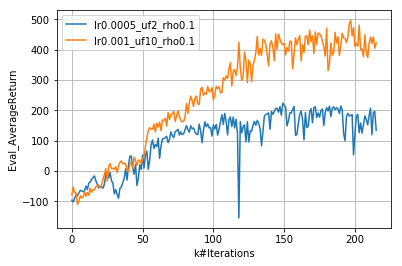
\includegraphics[width=.9\linewidth]{./5.png}
\caption{\textbf{Q5} DDPG for \texttt{HalfCheeah-v2}, with two different learning schedule}
\end{figure}

DDPG manages to solve this task and as you can see, given that

\begin{minted}[]{bash}
python run_hw4.py exp_name=q5_ddpg_hard_lr0.001_uf10  rl_alg=ddpg \
    env_name=HalfCheetah-v2 atari=false n_iter=100000 \
    learning_rate=0.001 policy_update_frequency=10

python run_hw4.py exp_name=q5_ddpg_hard_lr0.001_uf100 rl_alg=ddpg \
    env_name=HalfCheetah-v2 atari=false n_iter=100000 \
    learning_rate=0.001 policy_update_frequency=100
\end{minted}

\clearpage


\section{Question 6}
\label{sec:orgc5786a7}

\begin{figure}[htbp]
\centering
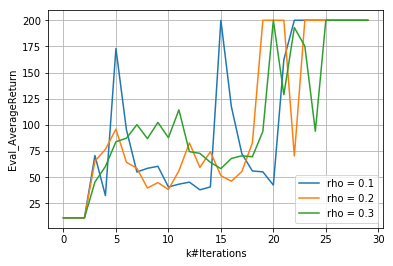
\includegraphics[width=.9\linewidth]{./61.png}
\caption{\textbf{Q6} TD3 for \texttt{InvertedPendulum-v2}, \texttt{td3\_target\_policy\_noise} ablations}
\end{figure}


\begin{figure}[htbp]
\centering
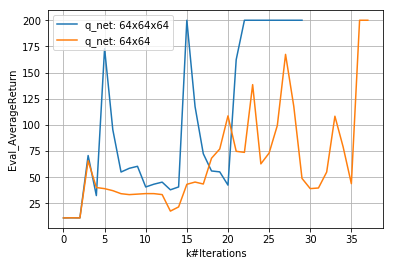
\includegraphics[width=.9\linewidth]{./62.png}
\caption{\textbf{Q6} TD3 for \texttt{InvertedPendulum-v2}, Q-network size ablations}
\end{figure}

\begin{minted}[]{bash}
python run_hw4.py exp_name=q6_td3_rho0.1 rl_alg=td3 \
    env_name=InvertedPendulum-v2 atari=false n_iter=30000 \
    learning_rate=0.001 td3_target_policy_noise=0.1

python run_hw4.py exp_name=q6_td3_rho0.2 rl_alg=td3 \
    env_name=InvertedPendulum-v2 atari=false n_iter=30000 \
    learning_rate=0.001 td3_target_policy_noise=0.2

python run_hw4.py exp_name=q6_td3_rho0.3 rl_alg=td3 \
    env_name=InvertedPendulum-v2 atari=false n_iter=30000 \
    learning_rate=0.001 td3_target_policy_noise=0.3

python run_hw4.py exp_name=q6_td3_rho0.1_shape2 rl_alg=td3 \
    env_name=InvertedPendulum-v2 atari=false n_iter=100000 \
    learning_rate=0.001 td3_target_policy_noise=0.1 n_layers_critic=2
\end{minted}

\clearpage


\section{Question 7}
\label{sec:org40d73b1}

\begin{figure}[htbp]
\centering
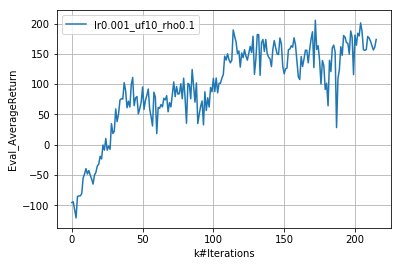
\includegraphics[width=.9\linewidth]{./7.png}
\caption{\textbf{Q7} TD3 for \texttt{HalfCheetah-v2}}
\end{figure}

\begin{minted}[]{bash}
python run_hw4.py exp_name=q7_td3_hard_lr0.001_uf10_rho0.1_shape3 \
    rl_alg=td3 n_layers_critic=3 \
    env_name=HalfCheetah-v2 atari=false n_iter=1000000 \
    learning_rate=0.001 policy_update_frequency=10 td3_target_policy_noise=0.1

python run_hw4.py exp_name=q7_td3_hard_lr0.0005_uf2_rho0.1_shape3 \
    rl_alg=td3 n_layers_critic=3 \
    env_name=HalfCheetah-v2 atari=false n_iter=1000000 \
    learning_rate=0.0005 policy_update_frequency=2 td3_target_policy_noise=0.1
\end{minted}

There is a huge difference between the performance of DDPG and TD3 in the task of \texttt{HalfCheetah-v2}, both in terms of the sample efficiency and in the overall pattern of learning (learning curves). This difference stems from the smoothing property of the noise added on top of the actions sampled from the policy, when forming the Q-network target update. This trick was introduces by TD3 to prevent the policy network to come up with hacky ways to exploit the structure of the imperfect Q-network, however, here this trick is somewhat unnecessary, as it introduces too much bias and apparently the Q-network is already in good shape in the context of this specific task. DDPG seems to be more sample efficient, at least in comparison with TD3 with \(\rho = 0.1\), i.e. the noise on top of target actions. Admittedly, TD3 is not tuned to the best of its abilities here, and would be jumping to conclusions to dismiss it as inferior to DDPG, solely based on this experiment.

\clearpage
\end{document}
